\documentclass{tufte-handout}
\usepackage[utf8]{inputenc}
\usepackage[russian]{babel}

\usepackage{amsmath}
\usepackage{amsfonts}
\usepackage{amssymb}
\usepackage{url}
\usepackage[pdftex]{graphicx}
%\usepackage[left=2cm,right=2cm,top=2cm,bottom=2cm]{geometry}


\DeclareMathOperator{\Var}{Var}
\DeclareMathOperator{\E}{E}



\title{Теория вероятностей: культурный код}
\author{Фольклор}
\date{\today}
\begin{document}

\maketitle

\section{Культурный код}

Сборник восхитительных задач по элементарной теории вероятностей. Эти задачи --- наша вероятностная ДНК.

\section{Фольклор и красота}


\begin{enumerate}
\item Задача о Сумасшедшей Старушке.

В самолете $100$ мест и все билеты проданы. Первой в очереди на посадку стоит Сумасшедшая Старушка. Сумасшедшая Старушка несмотря на билет садиться на случайно выбираемое место. Каждый оставшийся пассажир садится на своё место, если оно свободно и на случайное выбираемое место, если его место уже кем-то занято.

\begin{enumerate}
% \item Какова вероятность того, что все пассажиры сядут на свои места?
%\item Какова вероятность того, что второй пассажир в очереди сядет на своё место? 
\item Какова вероятность того, что последний пассажир сядет на своё место?
\item Чему примерно равно среднее количество пассажиров севших на свои места?
\end{enumerate}


\item Задача собирателя наклеек. Coupon collector's problem. 

Производитель чудо-юдо-йогуртов наклеивает на каждую упаковку одну из 50 случайно выбираемых наклеек. Покупатель собравший все виды наклеек получает приз от производителя. Пусть $X$ --- это количество упаковок йогурта, которое нужно купить, чтобы собрать все наклейки.

Найдите  $\E(X)$, $\Var(X)$

\item Спички Банаха. Banach's matchbox problem.

Польский математик Стефан Банах имел привычку носить в каждом из двух карманов пальто по коробку спичек. Всякий раз, когда ему хотелось закурить трубку, он выбирал наугад один из коробков и доставал из него спичку. Первоначально в каждом коробке было по $n$ спичек. Но когда-то наступает момент, когда выбранный наугад коробок оказывается пустым.

\begin{enumerate}
\item Какова вероятность того, что в другом коробке в этот момент осталось ровно $k$ спичек?
\item Каково среднее количество спичек в другом коробке?
\end{enumerate}


\item Равновесие Харди-Вайнберга. 

Предположим, что три возможных генотипа \verb|aa|, \verb|Aa| и \verb|AA| изначально встречаются с частотами $p_1$, $p_2$ и $p_3$, где $p_1+p_2+p_3=1$. Ген не сцеплен с полом, поэтому частоты $p_1$, $p_2$ и $p_3$ одинаковы для мужчин и для женщин. 
\begin{enumerate}
\item У семейных пар из этой популяции рождаются дети. Назовём этих детей первым поколением. Каковы частоты для трёх возможных генотипов в первом поколении? 
\item У семейных пар первого поколения тоже рождаются дети. Назовём этих детей вторым поколением. Каковы частоты для трёх возможных генотипов во втором поколении? 
\item Каковы частоты для трёх возможных генотипов в $n$-ном поколении?
\item Заметив явную особенность предыдущего ответа сформулируйте теорему о равновесии Харди-Вайнберга. Прокомментируйте утверждение: <<Любой рецессивный ген со временем исчезнет>>.
\end{enumerate}

\item Поляризация света.

Световая волна может быть разложена на две поляризованные составляющие, вертикальную и горизонтальную. Поэтому состояние отдельного поляризованного фотона может быть описано углом $\alpha$.\marginnote{На самом деле внутренний мир фотона гораздо разнообразнее.} Поляризационный фильтр описывается углом поворота $\theta$. Фотон в состоянии $\alpha$ задерживается поляризационным фильтром с параметром $\theta$ с вероятностью $p=\sin^2(\alpha-\theta)$ или проходит сквозь фильтр с вероятностью $1-p$, переходя при этом в состояние $\theta$. 

\begin{enumerate}
\item Какова вероятность того, что поляризованный фотон в состоянии $\alpha$ пройдёт сквозь фильтр с параметром $\theta=0$?
\item Имеется два фильтра и поляризованный фотон в состоянии $\alpha$. Первый фильтр --- с $\theta=0$, второй --- c $\theta=\pi/2$. Какова вероятность того, что фотон пройдет через оба фильтра?
\item Имеется три фильтра и поляризованный фотон в состоянии $\alpha$. Первый фильтр --- с $\theta=0$, второй --- c $\theta=\beta$, третий --- с $\theta=\pi/2$. Какова вероятность того, что фотон пройдет через все три фильтра? При каких $\alpha$ и $\beta$ она будет максимальной и чему при этом она будет равна?
\item Объясните следующий фокус. Фокусник берет два специальных стекла и видно, что свет сквозь них не проходит. Фокусник ставит между двумя стёклами третье, и свет начинает проходить через три стекла\marginnote{Как сделать <<секретный монитор>> своими руками, \url{http://www.youtube.com/watch?v=-ojbykV1zyc}}. 
\end{enumerate}


\item Истеричная певица

Начинающая певица дает концерты каждый день. Каждый ее концерт приносит продюсеру 0.75 тысяч евро. После каждого концерта певица может впасть в депрессию с вероятностью 0.5. Самостоятельно выйти из депрессии певица не может. В депрессии она не в состоянии проводить концерты. Помочь ей могут только цветы от продюсера. Если подарить цветы на сумму $0\le x\le 1$ тысяч евро, то она выйдет из депрессии с вероятностью $\sqrt{x}$. 

Какова оптимальная стратегия продюсера? 

\item Парадокс Симпсона.  Simpson's Paradox.

Два лекарства испытывали на мужчинах и женщинах. Каждый
человек принимал только одно лекарство. Общий процент людей,
почувствовавших улучшение, больше среди принимавших лекарство А.
Процент мужчин, почувствовавших улучшение, больше среди мужчин, принимавших лекарство В. Процент женщин, почувствовавших улучшение, больше среди женщин, принимавших лекарство В. 

Возможно ли это? 

\item Вовочку перевели из класса А в класс Б. Мог ли при этом возрасти средний балл по математике в обоих классах?

\item Злобный дракон поймал трех гномов. И решил поиграться с ними. Каждому гному он надевает с равными вероятностями черный или белый колпак. 
\marginnote{ --- Значит дракон --- это датчик случайных колпаков?} 


Гномы видят чужие колпаки, но не видят своих и не могут общаться после выдачи колпаков. Каждый гном может попытаться угадать цвет своего колпака, либо промолчать. Дракон отпустит гномов, если хотя бы один гном угадал цвет своего колпака, и никто не сделал ошибки. Если все одновременно промолчали, или кто-нибудь ошибся, то все гномы будут съедены. Перед игрой гномы могут договориться о стратегии игры.
\begin{enumerate}
\item Как им следует играть? Какова вероятность того, что они будут спасены?
\item Если от далекого спутника нужно получить один бит информации (<<да>> или <<нет>>), то, отправив три бита, можно не бояться того, что природа <<испортит>> один из них. Постройте этот простой код. Проведите аналогию с предыдущим пунктом. \marginnote{ --- Три гнома --- три бита?}
\end{enumerate}
Идея этой задачи используется не только при космической связи. Чтобы неглубокие царапины на компакт диске не вызывали потерь данных при записи используется код Рида-Соломона.
\marginnote{ --- А как звали третьего гнома?}

\item Париж, Людовик XIV, 1654 год, высшее общество говорит о рождении новой науки --- теории вероятностей. Ах, кавалер де Мере, <<fort honnete homme sans etre mathematicien>>\ldots \marginnote{<<благородный человек, хотя и не математик>>.} Старая задача, неправильные решения которой предлагались тысячелетиями (например, одно из неправильных решений предлагал изобретатель двойной записи, кумир бухгалтеров, Лука Пачоли) наконец решена правильно!


Два игрока играют в честную игру до шести побед. Игрок первым выигравший шесть партий (не обязательно подряд) получает 800 луидоров. К текущему моменту первый игрок выиграл 5 партий, а второй --- 3 партии. Они вынуждены прервать игру в данной ситуации.


Как им поделить приз по справедливости? 

\item На арене две команды гладиаторов,  $A$  и  $B$ . Каждый гладиатор обладает определенной силой, неизменной по ходу игры. Команды могут отличаться по количеству гладиаторов и их силе. Игра проходит в виде последовательных турниров, в каждом из которых участвует по одному гладиатору от каждой стороны. Если в очередном турнире встречаются гладиаторы с силами  $a$  и  $b$ , то вероятность победы первого определяется величиной  $\frac{a}{a+b} $ . Гладиатор, проигравший турнир, выбывает из игры, выигравший --- возвращается в команду. Гладиаторы не устают, но и не приобретают опыта. Стратегия команды предписывает, какого гладиатора выдвигать на очередной турнир в зависимости текущего состава команд. Игра ведется до полного выбывания из игры одной из команд.

Как выглядит оптимальная стратегия команды $A$?

\item В отличие от обычного гладиатора, у победившего гладиатора-вампира сила увеличивается на силу побежденного им гладиатора-вампира. В остальном правила поединка такие же, как в предыдущей задаче.

Как выглядит оптимальная стратегия команды $A$?

\item Маша и Саша играют в быстрые шахматы. У них одинаковый класс игры и оба предпочитают играть белыми, т.е. вероятность выигрыша белых  $p>0.5$. Партии играются до 10 побед. Первую партию Маша играет белыми. Она считает, что в следующей партии белыми должен играть тот, кто выиграл предыдущую партию. Саша считает, что ходить белыми нужно по очереди. При каком варианте правил у Маши больше шансы выиграть?

\item Гадалка

Маша пишет на бумажках два любых различных натуральных числа по своему выбору. Одну бумажку она прячет в левую руку, а другую --- в правую. Саша выбирает любую Машину руку. Маша показывает число, написанное на выбранной бумажке. Саша высказывает свою догадку о том, открыл ли он большее из двух чисел или меньшее. Если Саша не угадал, то Маша выиграла.

Существует ли у Саши стратегия, гарантирующая ему выигрыш с вероятностью строго более 50\%, даже будучи известной Маше?

\item Больший кусок окружности

Аня хватается за верёвку в форму окружности в любой точке. Дальше мы делаем в случайных местах два разреза веревки. Аня забирает себе тот кусок, за который держится. Боря забирает оставшийся кусок. Выигрыш каждого равен длине полученной им верёвки. 
\begin{enumerate}
\item Чему равен средний выигрыш каждого игрока?
\item  Вероятность того, что у Ани верёвка длиннее?
\end{enumerate}


\item Судьба Дон-Жуана. 

У Дон-Жуана $n$  знакомых девушек, и их всех зовут по-разному. Он пишет
им $n$  писем, но по рассеянности раскладывает их в конверты
наугад. Случайная величина $X$ обозначает количество девушек, получивших письма, адресованные лично им.

\begin{enumerate}
\item Найдите $\E(X)$, $\Var(X)$
\item Какова при большом $n$ вероятность того, что хотя бы одна девушка получит письмо, адресованное ей?
\end{enumerate}



\item Саша и Маша подкидывают монетку до тех пор, пока не выпадет
последовательность РОО или ОOР. Если игра закончится выпадением
РОО, то выигрывает Саша, если ОOР, то --- Маша. 
\begin{enumerate}
\item Какова вероятность того, что победит Маша?
\item Сколько бросков в среднем продолжается игра?
\end{enumerate}

\item Илье Муромцу предстоит дорога к камню. От камня начинаются ещё три дороги. Каждая из тех дорог снова оканчивается камнем. И от каждого камня начинаются ещё три дороги. И каждые те три дороги оканчиваются камнем\ldots И так далее до бесконечности. На каждой дороге живёт трёхголовый Змей Горыныч. Каждый Змей Горыныч бодрствует независимо от других с вероятностью (хм, Вы не поверите!) одна третья. У Василисы Премудрой существует Чудо-Карта, на которой видно, какие Змеи Горынычи бодрствуют, а какие --- нет. Какова вероятность того, что Василиса Премудрая сможет найти на карте  бесконечный жизненный путь Ильи Муромца проходящий исключительно мимо спящих Змеев Горынычей?

\item У тети Маши --- двое детей разных возрастов. Вероятности рождения мальчика и девочки равны. 
\begin{enumerate}
\item Какова вероятность того, что у тёти Маши оба ребёнка --- мальчики, если известно, что у неё хотя бы один ребёнок --- мальчик?
\item Какова вероятность того, что у тёти Маши оба ребёнка --- мальчики, если известно, что у неё хотя бы один ребёнок --- мальчик водолей по гороскопу?
\end{enumerate}

\item Buffon's needle problem

Плоскость разлинована параллельными линиями через каждый сантиметр. Случайным образом на эту плоскость бросается иголка длины $a<1$. 

\begin{enumerate}
\item Какова вероятность того, что иголка пересечёт какую-нибудь линию?
\item Предложите вероятностный способ оценки числа $\pi$
\end{enumerate}

\item Мартышка и Шекспир

Мартышка наугад нажимает клавиши на печатающей машинке. 


\begin{enumerate}
\item Какова вероятность того, что она рано или поздно напечатает полное собрание сочинений Шекспира? Льва Толстого?
\item Обозначим количество нажатий до появления слова <<АБРАКАДАБРА>> за $X$. Найдите $\E(X)$ и $\Var(X)$.
\end{enumerate}


\begin{marginfigure}
  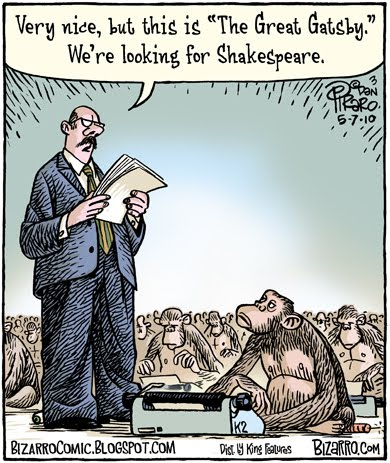
\includegraphics[width=5cm]{gatsby}
  \caption{Задача о <<бесконечных обезьянах>>, infinte-monkey problem. }
\end{marginfigure}

\item Парадокс инспектора

Автобусы приходят на остановку согласно пуассоновскому потоку в среднем один раз в час. Вася приходит на остановку в случайный момент времени и садится на первый пришедший автобус. 

\begin{enumerate}
\item Сколько Васе в среднем предстоит ждать автобуса?
\item Сколько в среднем прошло времени от последнего пришедшего автобуса до Васиного появления?
\item Чему равна средняя продолжительность интервала между автобусом, на который сядет Вася, и предыдущим?
\item Чему равна средняя продолжительность интервала между автобусом, на который сядет Вася, и следующим?
\item Маша не любит набитые битком автобусы и никогда не торопится, поэтому, придя на остановку, всегда пропускает один автобус и садится на следующий. Она считает, что на него в среднем сядет меньше людей. Права ли она?
\end{enumerate}

\item Спящая красавица

Спящая красавица согласилась принять участие в научном
эксперименте. В воскресенье её специально уколют веретеном. Как
только она заснёт, будет подброшена правильная монетка. 


Если
монетка выпадет орлом, то спящую красавицу разбудят в понедельник
и спросят о том, как выпала монетка. 


Если монетка выпадет решкой,
то спящую царевну разбудят в понедельник, спросят о монетке, снова
уколют веретеном, разбудят во вторник и снова спросят о монетке.
Укол веретена вызывает легкую амнезию, и красавица не сможет
определить, просыпается ли она в первый раз или во второй.


Красавица только-только проснулась. Вспомнила правила эксперимента, и услышала вопрос исследователя: <<Ваше Высочество, так как же выпала монетка?>>
\begin{enumerate}
\item Как следует отвечать красавице, если за каждый верный ответ ей
дарят молодильное яблоко?
\item Как следует отвечать красавице, если за неверный ответ её тут
же превращают в тыкву?
\item Отвечая на вопрос исследователя Спящая Красавица задумалась, а какова вероятность того, что сегодня понедельник. Как ты думаешь?
\end{enumerate}


Решение: 


<<Сегодня понедельник>> "--- это \textbf{не} событие. Вероятность не
определена. Это функция от времени.

Вероятность того, что монетка выпала орлом, равна $0{,}5$. Поэтому ей
всё равно, как отвечать, если наказанием является превращение в
тыкву, и нужно отвечать: <<Решка!>> "--- если наградой является
молодильное яблоко. Предположим, что красавица максимизирует
ожидаемое количество молодильных яблок. 


\item Monty-Hall 

Есть три закрытых двери. За двумя из них --- по козе, за третьей автомобиль. Вы выбираете одну из дверей. Допустим, Вы выбрали дверь А. Ведущий шоу, чтобы поддержать интригу, не открывает сразу выбранную Вами дверь. Сначала он открывает одну из дверей не выбранных Вами, причем снова ради интриги ведущий не открывает сразу и дверь с автомобилем. Допустим, ведущий открыл дверь B. И в этот момент он предлагает Вам изменить ваш выбор двери.

Имеет ли смысл изменить свой выбор?

\begin{figure*}
  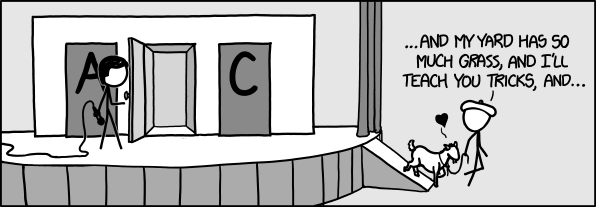
\includegraphics[width=17cm]{monty_hall}
  \caption{A few minutes later, the goat from behind door C drives away in the car. \url{http://xkcd.com/1282/}}
\end{figure*}


\item Monty-Hall версия

Трое студентов, Аня, Боря и Василиса, сдавали комиссию по теории вероятностей и ещё не знают своих оценок. Им объявили, что зачёт получили двое из трёх. В перерыве перед объявлением оценок Боря подходит к председателю:

--- Иван Иванович, раз зачёт получили двое из трёх, значит хотя бы у одной из девушек есть зачёт. Вы мне можете назвать имя одной из девушек, получившей зачет?

--- Василиса получила.

Какова условная вероятность того, что Боря получил зачёт, если принимать во внимание информацию от Ивана Ивановича?



\end{enumerate}

\section{Опорные задачи}

\begin{enumerate}
\item Стрелок попадает по мишени с вероятностью 0.3. Какова вероятность того, что до третьего промаха у него будет 5 выстрелов?

\item Расстояние от пункта A до B автобус проходит за 2 мин, а пешеход — за 20 мин. Интервал движения автобусов 30 мин. Вы подходите в случайный момент времени к пункту A и отправляетесь в B пешком. 

\begin{enumerate}
\item Какова вероятность того, что в пути Вас догонит очередной автобус?
\item Сколько в среднем времени Вы будете добираться, если проходящий мимо автобус обязательно Вас подбирает?
\end{enumerate}

% 18/30, примерно 14 минут


\item Ген карих глаз доминирует ген синих. Т.е. у носителя пары bb
глаза синие, а у носителя пар BB и Bb --- карие. У диплоидных
организмов (а мы такие :)) одна аллель наследуется от папы, а одна
--- от мамы. В семье у кареглазых родителей два сына --- кареглазый и
синеглазый. Кареглазый женился на синеглазой девушке. Какова
вероятность рождения у них синеглазого ребенка?


\item Задача о полосе невезения

За неделю Аннушка семь раз пролила масло. Какова вероятность того, что она проливала масло каждый день?



\end{enumerate}

\section{Черновые размышления :)}

Сумасшедшая старушка  ок

Спички Банаха  ок

Наклейки ок

Дон-Жуан ок

Разборчивая невеста (\url{http://en.wikipedia.org/wiki/Secretary_problem})

Два конверта

Монти-Холл + Картинка от Рэнделла

Обезьяны и Шекспир (Абракадабра) ok

Двойное зеро на рулетке (вероятность выигрыша, сравнить с одним зеро)

ООР или РОО ок

Триэль

нетранзитивные рулетки

сколько теории игр включать? 

Две выигрышных игры

Парадокc инспектора ок

Гороскоп и пол ребенка ок

Гадалка и выбор наибольшего числа ok 

Задача о спящей красавице


Нестандартные задачи ??? ()

Автобус догоняет по дороге (вероятность и среднее) ok

певица и депрессия ok

удвоение ставки --- броуновское движение


Методы: ???

Первый шаг

Разложение в сумму --- Разделяй и властвуй

Большая сила о-малых

Матрешки --- (условное математическое ожидание)

Холмс, это невероятно! (Вероятностная интерпретация)

Как сварить мартингал (теорема Дуба)

Свернулся колечком (задачи на равномерное на отрезке)


Сюжеты: ????

Пуассоновский поток

Броуновское движение


Источники:

Феллер, Блом, Секей, 
\url{http://new.math.msu.su/department/probab/olimpia/olimpia.htm}

\url{https://www.math.ucdavis.edu/~gravner/MAT135A/resources/chpr.pdf}

\url{http://www.teorver.ru/newkatalog/1193689162.pdf}



\end{document}